\documentclass[
    10pt,
    aspectratio=169,
    xcolor={dvipsnames},
    % hyperref={colorlinks=true,linkcolor=blue,urlcolor=blue}
]{beamer}


\renewcommand{\familydefault}{\rmdefault}

\usetheme{metropolis}

\usepackage[english]{babel}
\usepackage{subcaption}
\usepackage{graphicx}

\title{The Doomsday Argument}
\author{Meesum Qazalbash}
\institute{Group 5}
\date{\today}

\begin{document}

\frame{\titlepage}

\begin{frame}
    \frametitle{Intorduction}
    It was first given by an astrophysicist \textbf{Brandon Carter} in early 1990s, and independently by \textbf{Richard Gott} and \textbf{H. Nielsen}. Later on it was popularized by \textbf{John Leslie} in his series of publication.

    \begin{figure}
        \centering
        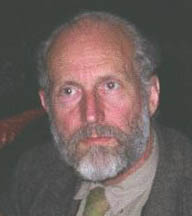
\includegraphics[width=0.2\textwidth]{BrandonCarter.jpeg}
        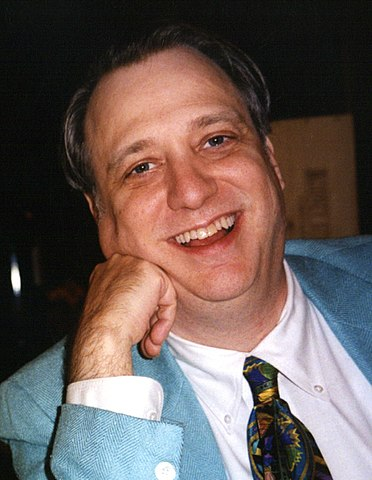
\includegraphics[width=0.2\textwidth]{372px-JRichardGott1989.jpeg}
        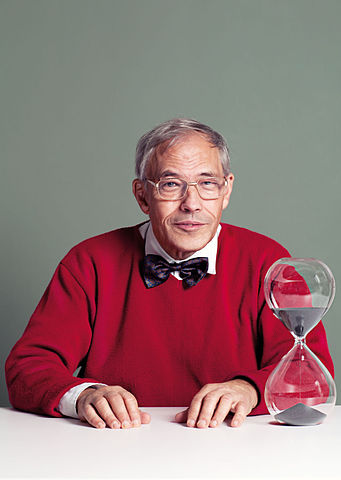
\includegraphics[width=0.2\textwidth]{341px-Holger_bech.jpeg}
        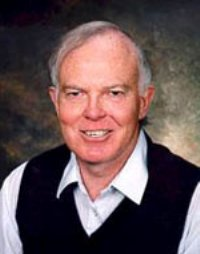
\includegraphics[width=0.2\textwidth]{John-Leslie.jpeg}
        \caption{From left to right, Brandon Carter, Richard Gott, Holger Bech Nielsen, and John Leslie}
    \end{figure}
\end{frame}

\begin{frame}
    \frametitle{History}
    When Richard Gott visited the Berlin Wall in 1969, he was curious to know how long it would last. He came up with a simple formula to predict the future of the wall. He assumed that he was visiting the wall at a random time during its existence. There has been 8 years since the wall was built, and it is still standing. So, he predicted that the wall would last for atleast 2 years and 8 months but atmost 24 years. The wall was torn down in 1989, 20 years after he visited it. This formula is now known as \textbf{Copernican Principle}.
\end{frame}

\begin{frame}
    \frametitle{Argument}
    The argument says, if we sample a random human from the set of all humans that have ever lived, then the probability that the sampled human is among the last 5\% of humans ever to be born is close to 95\%.
\end{frame}

\begin{frame}[allowframebreaks]
    \frametitle{Explaination}
    Let's hypothesize that there are two different populations of total human that would ever live on the face of earth, i.e. \(n\) and \(N\), where \(n<N\). Let us consider the fact that the random human we have sampled has ordinal \(t\). Then the probabilities would be,
    \[P(t|T=n)=\frac{1}{n}\qquad\qquad P(t|T=N)=\frac{1}{N}\]
    Each senario is equally likely, so the probability of sampling a human from the first population or second population is,
    \[P(T=n)=P(T=N)=\frac{1}{2}\]
    By applying Bayes' theorem,
    \begin{align}
        P(T=n|t) & =\frac{P(t|T=n)P(T=n)}{P(t|T=n)P(T=n)+P(t|T=N)P(T=N)}                                           \\
                 & =\frac{\frac{1}{n}\times\frac{1}{2}}{\frac{1}{n}\times\frac{1}{2}+\frac{1}{N}\times\frac{1}{2}} \\
                 & =\frac{N}{N+n}
    \end{align}
    Similarly,
    \[P(T=N|t)=\frac{n}{N+n}\]
    We assumed that,
    \begin{align}
             & n                   < N                      \\
        \iff & 2n             < N+n                         \\
        \iff & \frac{n}{N+n}  < \frac{1}{2}                 \\
        \iff & P(T=N|t)       < \frac{1}{2}                 \\
        \iff & P(T=N|t) + P(T=n|t) < \frac{1}{2} + P(T=n|t) \\
        \iff & 1 < \frac{1}{2} + P(T=n|t)                   \\
        \iff & \frac{1}{2} < P(T=n|t)
    \end{align}
\end{frame}

\begin{frame}
    \frametitle{Inference}
    We get two important results from the above argument,
    \[P(T=N|t) < \frac{1}{2} < P(T=n|t)\]
    We can infere that, chance that there is a large number of population that would be after the sampled human is very low, more precisely less than 50\%. And the chances that there is a small number of population that would be after the sampled human is very high, more precisely more than 50\%.

    \begin{center}
        \textbf{End is near.}
    \end{center}
\end{frame}


\begin{frame}
    \frametitle{Criticism}
    \begin{itemize}
        \item Subjective assumption about one's own birth rank.
        \item Lack of consideration for technological advancements.
        \item Uncertain population growth.
    \end{itemize}
\end{frame}

\begin{frame}
    \frametitle{Conclusion}
    \begin{itemize}
        \item It is a controversial argument.
        \item It uses statistical inference to predict the future.
        \item It is based on the Copernican Principle.
    \end{itemize}
\end{frame}

\begin{frame}
    Questions
\end{frame}

\begin{frame}
    Thank you
\end{frame}

\end{document}
